\documentclass[12pt, a4paper, oneside]{report}

\usepackage{amsmath}
\usepackage{esint}
\usepackage{geometry}
\usepackage{graphicx}
\usepackage{subcaption}
\usepackage{cleveref}
\usepackage{ctex}
\usepackage{listings}
\usepackage{color}
\definecolor{dkgreen}{rgb}{0,0.6,0}
\definecolor{gray}{rgb}{0.5,0.5,0.5}
\definecolor{mauve}{rgb}{0.58,0,0.82}
\lstset{frame=tb,
	language=Python,
	aboveskip=3mm,
	belowskip=3mm,
	showstringspaces=false,
	columns=flexible,
	basicstyle={\small\ttfamily},
	numbers=left,%设置行号位置none不显示行号
	numberstyle=\tiny\color{gray},
	keywordstyle=\color{blue},
	commentstyle=\color{dkgreen},
	stringstyle=\color{mauve},
	breaklines=true,
	breakatwhitespace=true,
	escapeinside=``,%逃逸字符(1左面的键),用于显示中文例如在代码中`中文...`
	tabsize=4,
	extendedchars=false %解决代码跨页时,章节标题,页眉等汉字不显示的问题
}
% 导言区

\title{Report 2: Colorization Using Optimization}
\author{Chihao Shen 121020163}
\CTEXoptions[today=old]
\geometry{left=2cm,right=2cm,top=2.5cm,bottom=2.5cm}




\begin{document}
	
	\rmfamily
	\maketitle
	
	\songti 
	
	\section{任务描述}
	
	优化上色,将一张黑白的灰度图片转化为彩色图片。要求在需要上色的区域涂上和区域颜色相类似单色,输入这张局部上色的图片和原来的灰度图片,即可输出一张与符合观感的上色后的彩色图片。
	
	\centerline{	
		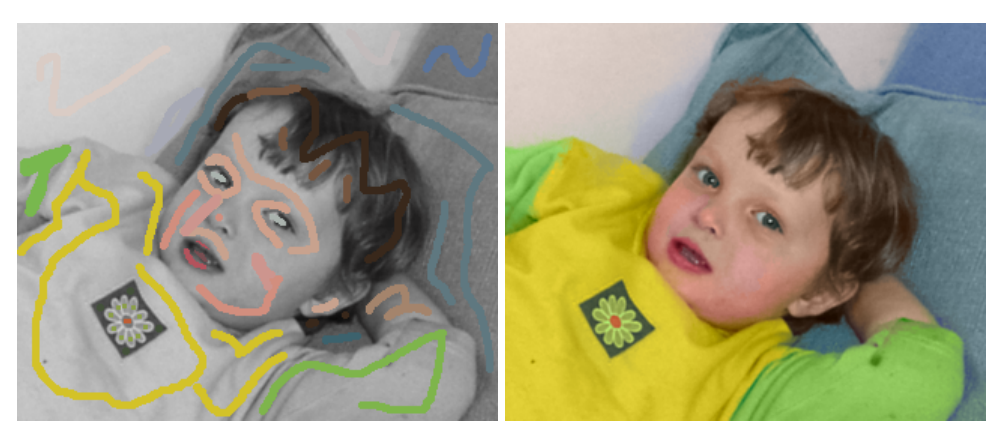
\includegraphics[scale=0.3]{task.png}
	}
	
	\section{理论基础}
	由于传统的上色方法需要将图像分为不同区域,再给区域分别上色,不但十分麻烦,部分区域由于不能进行很好的分割还会导致串色的现象,因此本文采用了一种新的优化方法。在黑白图片中,我们能够获取到的信息是图像的Y值 (Luminance (Intensity),亮度),由经验可得,亮度相似的地方颜色也较为相似,基于这一假设,U值和V值(Chrominance,色度)与Y值高度相关。因此,作者给出了一个基于Y值相似度权重的表达式:
	$$\min\sum_r\left(U\left(\mathbf{r}\right) - \sum_{\mathbf{s}\in
	N\left(\mathbf{r}\right)}w_{\mathbf{rs}}U\left(\mathbf{s}\right)\right)^2$$
	
	其中,$\mathbf{r}$为当前像素,$U\left(\mathbf{r}\right)$为当前像素的U值,为待求量。$\mathbf{s}$属于其邻域的八个像素。$w_{\mathbf{rs}}$代表邻域像素$\mathbf{s}$相对于中心像素$\mathbf{r}$的比重系数,由$\mathbf{r}$和$\mathbf{s}$间Y值的相似程度决定,相似程度越大,邻域像素的$w$值就越大,该邻域像素U值的占比就越大,V值同理。这就满足了亮度越相似,色度也越相似的假设。同时,解得各个邻域像素的比重系数后,需要平衡到总和为1以满足拟合的有效性。由于式中的U值和V值都为未知量,我们需要给出一张局部上色的图像,通过已知的给定部分像素的初始值,来计算剩余像素的U值和V值。
	
	基于这个表达式,作者给出两种确定比重系数$w$的方法。第一种是基于相邻两个像素的Y值平方差的正态分布函数:
	$$w_{\mathbf{rs}}\propto e^{-\left(Y\left(\mathbf{r}\right) - Y\left(\mathbf{s}\right)\right)^2 / 2\sigma_{\mathbf{r}}^2}$$
	
	第二种是基于Y值归一化相关性而得出的函数:
	$$w_{\mathbf{rs}}\propto 1 + \frac{1}{\sigma_{\mathbf{r}}^2}\left(Y\left(\mathbf{r}\right) - \mu_{\mathbf{r}}\right)\left(Y\left(\mathbf{s}\right) - \mu_{\mathbf{r}}\right)$$
	
	其中,$\sigma_{\mathbf{r}}$为中心像素$\mathbf{r}$及其邻域像素(最多为$3\times3$共9个像素的窗格)Y值的方差,$\mu_{\mathbf{r}}$为这些像素Y值的平均值。
	
	第一种方法是较为常用的图像分割的算法,而第二种则是基于一篇名为Multi-sensor Super-Resolution的论文,其中表述了RGB通道的变化在一张图像的各个像素及其邻域中具有高度的相关性,由于YUV是RGB的线性表达式,因此可以得出亮度Y和色度UV有高度的相关性,即在中心像素及其邻域中,满足$U\left(/V\right) = aY + b$,代入邻域的U (/V)值和Y值,即可解得系数a和b,代入中心像素的Y值,就能得到U和V的值。而该式经简化后即为第二种方法的相关性函数。
	
	在实际计算的过程中,最小化权重表达式即让权重表达式等于0,即$U\left(\mathbf{r}\right) - \sum_{\mathbf{s}\in
			N\left(\mathbf{r}\right)}w_{\mathbf{rs}}U\left(\mathbf{s}\right) = 0$,提取局部上色的像素的U和V值(上色的像素无须满足该式,因为它是人为给定的初始值而不是拟合的),根据Y值计算出的$w$比重系数,通过线性方程解出其余位置的U值和V值,同时需要调整方差$\sigma$使图像的效果最佳。
		
	\centerline{
	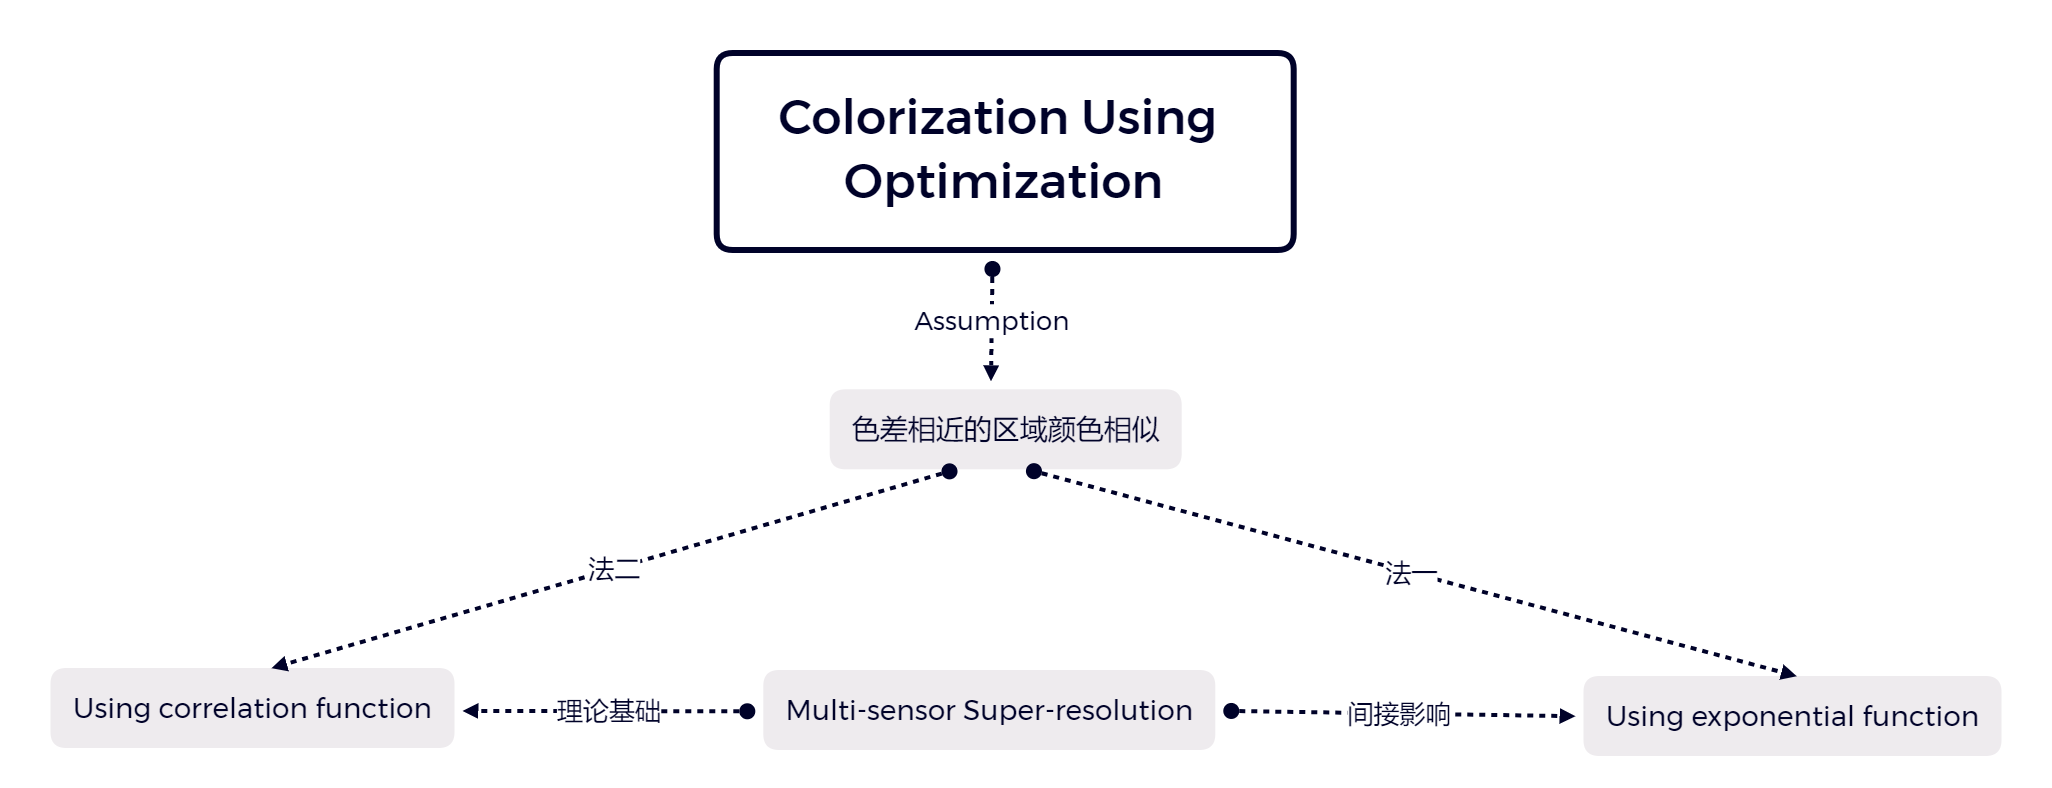
\includegraphics[scale=0.25]{Colorization Using Optimization.png}	
	}
	
	
	接下来取一张$2\times3$的简化模型来说明具体的计算过程。首先我们先根据已知的Y值计算出各处的$w$值。接下来假设U值为$\left[ \begin{array}{ccc}
		x1 & x2 & x3\\
		x4 & x5 & x6
	\end{array}\right]$,我们将x1处上色为u1,x5处上色为u5,将剩下四个像素分别代入上述权重表达式,得到一个线性系统:
	$$\left[ \begin{array}{cccccc}
		1 & 0 & 0 & 0 & 0 & 0\\
		-w_{21} & 1 & -w_{23} & -w_{24} & -w_{25} & -w_{26}\\
		0 & -w_{32} & 1 & 0 & -w_{35} & -w_{36}\\
		-w_{41} & -w_{42} & 0 & 1 & -w_{45} & 0\\
		0 & 0 & 0 & 0 & 1 & 0\\
		0 & -w_{62} & -w_{63} & 0 & -w_{65} & 1\\
	\end{array}\right]
	\left[ \begin{array}{c}
		x1\\
		x2\\
		x3\\
		x4\\
		x5\\
		x6\end{array}\right] = 
	\left[ \begin{array}{c}
		u1\\
		0\\
		0\\
		0\\
		u5\\
		0\end{array}\right]
		$$
	通过这个线性系统,我们就能解出剩下的未知数,从而得到整个模型的U值。从中也能发现,无论怎么更改局部上色的位置或是颜色,我们总能得到一组对应解,由此可以说明最终拟合出的图像的颜色是由局部上色图像的位置和颜色决定的,而不具有唯一性,如下图所示:
	\centerline{
	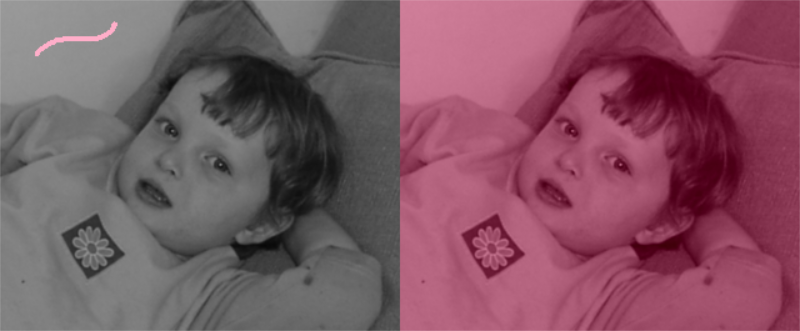
\includegraphics[scale=0.6]{baby_colorized1.png}
	}
	
	因此,我们可以根据个人的意愿将图片上色成自己所需要的样式。
	
	推广至一般,我们就能获取每个未知像素的U值和V值,最后再转化为RGB时要注意值域,超出1的保留至1,小于0的保留到0(OpenCV自动保留),即可解出上色后的图像。
	
	该方法的应用领域也很广,不但能对黑白图片进行上色,还具有对彩色图片重新着色,对黑白视频进行上色等应用。
	
	

	\section{代码实现}
	\subsection{代码说明}
	\noindent 库:numpy, OpenCV, sparse
	
	和任务1一样,我们依旧采用OpenCV获取和展示图片,并采用sparse稀疏矩阵来构造方程组,降低空间复杂度,提高计算效率。在实际测试中,使用正态分布函数时,将$\sigma_{\mathbf{r}}^2$的值缩小为方差的0.3倍左右,能使渲染出的效果最佳化。使用相关性函数时,笔者给出两种解决方案。由于相关性的线性函数对方差比较敏感,因此第一种是将$\sigma_{\mathbf{r}}^2$的值放大为方差的1.5倍缩小斜率,防止出现由于舍入而造成的大面积单色色块;第二种是将$\sigma_{\mathbf{r}}^2$的值放大为方差的1.00001倍(若$\sigma_{\mathbf{r}}^2$为方差,由于小数精度有限的问题,部分计算出的比重系数会舍入到0,导致最后矩阵出现计算错误),并将比重系数中所有的负数值变为原来的0.1倍,同样也可以防止单色色块的出现。但是这两种方法的效果比较一般,会出现部分溢色的现象。
	
	本代码需要根据提示分别输入一张黑白灰度图像以及对该图像局部上色后的图像的地址(最好采用bmp的图片格式,jpg会对图像颜色进行修改和压缩,使局部上色图像的上色位置出现渐变颜色,影响最后效果的呈现),并选择比重函数的类型,输入Y采用正态分布函数,输入N采用相关性函数,输入其它给出无效输入的提示。
	
	在演示结束后,笔者将会给出该上色方案存在的一些小的缺陷和问题。
	
	
	
	\subsection{代码}
	
	\begin{lstlisting}
import cv2
import time
import numpy as np
from scipy.sparse import csr_matrix
from scipy.sparse.linalg import spsolve

NUM_IN_WINDOW = 9
"""
NUM_IN_WINDOW: 一个窗格内的像素个数
"""


def colorization(p_original, p_marked, p_type):
	"""
	优化上色算法
	:param p_original: 原始黑白图片,格式为uint8
	:param p_marked: 带标记的图片,格式为uint8
	:param p_type: 比重函数的选择
	:return: 上色后的图片
	"""

	# 先转换为32位浮点类型方便计算
	p_original = p_original.astype(np.float32) / 255
	p_marked = p_marked.astype(np.float32) / 255
	
	# 转换为YUV格式
	p_original = cv2.cvtColor(p_original, cv2.COLOR_BGR2YUV)
	p_marked = cv2.cvtColor(p_marked, cv2.COLOR_BGR2YUV)
	
	# 判断像素值是否被标记
	# abs()防止原数组三个数一正一负相加刚好等于0的情况
	is_marked = abs(p_original - p_marked).sum(2) != 0
	
	# 创建相同大小的零矩阵,存放原始黑白图片的Y值和标记后图片的UV值
	YUV_comb = np.zeros(p_original.shape)
	YUV_comb[:, :, 0] = p_original[:, :, 0]
	YUV_comb[:, :, 1] = p_marked[:, :, 1]
	YUV_comb[:, :, 2] = p_marked[:, :, 2]
	
	# 获取宽高和图像大小
	height = p_original.shape[0]
	width = p_original.shape[1]
	image_size = height * width
	
	# 建立下标矩阵
	# order='F',为竖着读取竖着填充
	indices = np.arange(image_size).reshape(height, width, order='F').copy()
	
	# 最大像素接触数量为一个窗格的数量乘上图像像素个数
	max_pxls = image_size * NUM_IN_WINDOW
	
	# 按最大像素接触数量建立max_pxls * max_pxls稀疏矩阵
	# row_indices存放权重系数及其中心像素对应的线性方程组的行下标
	# col_indices存放权重系数及其中心像素在该线性方程组中的列下标
	# values存放权重系数及其中心像素在线性方程中的系数1
	# 三者一一对应
	row_indices = np.zeros(max_pxls)
	col_indices = np.zeros(max_pxls)
	values = np.zeros(max_pxls)
	
	index = 0  # 存放权重系数相关值的三个数组的下标
	current_pxl_index = 0  # 当前中心像素下标
	
	# 遍历图中每个像素,计算对应各个方向权重
	for col in range(width):
		for row in range(height):
			
			# 如果没有被标记
			if not is_marked[row, col]:
				window_index = 0  # 当前3 * 3窗格内的下标
				window_intst = np.zeros(NUM_IN_WINDOW)  # 存放每个下标对应的Y值
				
				# 遍历窗格内的各个像素,记录对应Y值
				for lcl_col in range(max(0, col - 1), min(col + 2, width)):
					for lcl_row in range(max(0, row - 1), min(row + 2, height)):
						
						# 不为中心像素时
						if lcl_col != col or lcl_row != row:
							row_indices[index] = current_pxl_index  # 记录周围像素对应中心像素的下标
							col_indices[index] = indices[lcl_row, lcl_col]  # 记录周围像素下标
							window_intst[window_index] = YUV_comb[lcl_row, lcl_col, 0]  # 记录周围像素Y值
							
							index += 1
							window_index += 1
				
				center_intst = YUV_comb[row, col, 0].copy()  # 中心像素Y值
				window_intst[window_index] = center_intst  # 记录中心像素Y值
				
				# 计算方差(包含中心)
				mean = np.mean(window_intst[0:window_index + 1])
				variance = np.mean((window_intst[0:window_index + 1] - mean) ** 2)
				window_weight = np.zeros(NUM_IN_WINDOW - 1)  # 存放对应周围像素的比例系数
				
				# 采用正态分布函数
				if p_type == 'Y':
					# 非零时,降低方差,给予相同或相似的像素更多比重
					# 为零时,比重都相同,不受方差影响,因此方差可以为任何值,这里赋值为1
					sigma_sqr = 1 if variance == 0 else 0.3 * variance
					
					# 计算比例系数
					window_weight[0:window_index] = np.exp(
					-((window_intst[0:window_index] - center_intst) ** 2) / (2 * sigma_sqr))
				
				# 采用相关性函数
				elif p_type == 'N':
					# 非零时,
					# 法一:由于相关性函数对数据十分敏感,所以增大方差,降低斜率
					# sigma_sqr = 1 if variance == 0 else 1.5 * variance
					# 法二:在保证数据有效
					# (不由于舍入规则使一些数据变为0)的情况下,减小负数部分的比重
					# 防止出现YUV转RGB时溢出导致出现大面积单色块的情况
					sigma_sqr = 1 if variance == 0 else 1.00001 * variance
					
					# 计算比例系数
					window_weight[0:window_index] = 1 + (window_intst[0:window_index] - mean) * (
					center_intst - mean) / sigma_sqr
					
					# 减小负数部分的比重
					for i in range(window_index):
						if window_weight[i] < 0:
							window_weight[i] = window_weight[i] / 10
				
				# 输入错误
				else:
					return
				
				# 使比例系数平衡到1
				window_weight[0:window_index] = window_weight[0:window_index] / np.sum(
				window_weight[0:window_index])
				
				values[index - window_index:index] = -window_weight[0:window_index]  # 记录比例系数
				
			# 记录当前的中心像素
			row_indices[index] = current_pxl_index
			col_indices[index] = current_pxl_index
			values[index] = 1
			index += 1
			current_pxl_index += 1
			
	# 去除空元素位
	values = values[0:index]
	col_indices = col_indices[0:index]
	row_indices = row_indices[0:index]
	
	# 建立稀疏矩阵,大小取image_size * image_size,建立等式右侧值
	A = csr_matrix((values, (row_indices, col_indices)), shape=(image_size, image_size))
	b = np.zeros(image_size)
	
	# 将判断标记像素数组变成一维
	is_marked = is_marked.reshape(image_size, order='F')
	
	# 返回判断标记像素数组中非零元素的下标索引
	marked_indices = np.nonzero(is_marked)
	
	# 新建要输出的将要上色的图片
	colorized = np.zeros(YUV_comb.shape)
	# 先复制亮度值
	colorized[:, :, 0] = YUV_comb[:, :, 0]
	
	# 分别计算U和V
	for i in [1, 2]:
		chrominance = YUV_comb[:, :, i].reshape(image_size, order='F').copy()
		b[marked_indices] = chrominance[marked_indices]  # 给标记的像素赋值
		res = spsolve(A, b)
		colorized[:, :, i] = res.reshape(height, width, order='F').copy()
	
	# 转换BGR,转换前要满足float32的类型
	colorized = colorized.astype(np.float32)
	colorized = cv2.cvtColor(colorized, cv2.COLOR_YUV2BGR)
	
	return colorized
	

def main():
	# 导入图像
	original_file = input('Enter original file name: ')
	marked_file = input('Enter marked file name: ')
	func_type = input("Enter 'Y' for exponential weighting function. "
	"Enter 'N' for correlation weighting function: ")
	original = cv2.imread(original_file)
	marked = cv2.imread(marked_file)
	
	# 处理
	start_time = time.time()
	colorized_pic = colorization(original, marked, func_type)
	
	# 输入无效
	if colorized_pic is None:
		print('Invalid input for weighting function!')
		return
	end_time = time.time()
	print('It spends {time} seconds.'.format(time=end_time - start_time))
	
	# 展示
	cv2.imshow('tgt', colorized_pic)
	cv2.waitKey(0)
	cv2.destroyAllWindows()


if __name__ == '__main__':
	main()
	\end{lstlisting}
	\noindent 代码见:https://github.com/StevenShen3641/colorization\_using\_optimization
	
	\noindent 上色:
	
	\noindent Original file: 
	
	\centerline{
	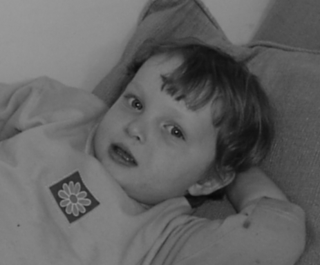
\includegraphics[scale=0.5]{baby.png}}
	
	\noindent Marked file:
	
	\centerline{
	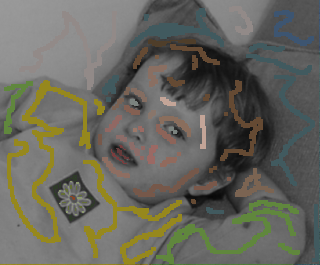
\includegraphics[scale=0.5]{baby_marked.png}}
	 
	\noindent Weighting function: Y / N
	

	\noindent Result: 
	
	\centerline{
	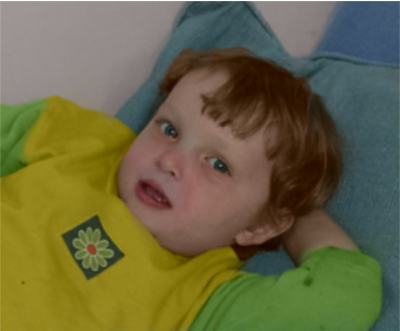
\includegraphics[scale=0.65]{baby_colorized.png}
	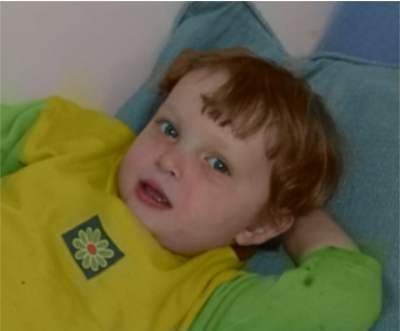
\includegraphics[scale=0.65]{baby_colorized3.png}}
	

	
	\noindent 用时:2.73s / 2.97s
	
	\noindent 重新着色:
	
	\noindent Original file: 
	
	\centerline{
		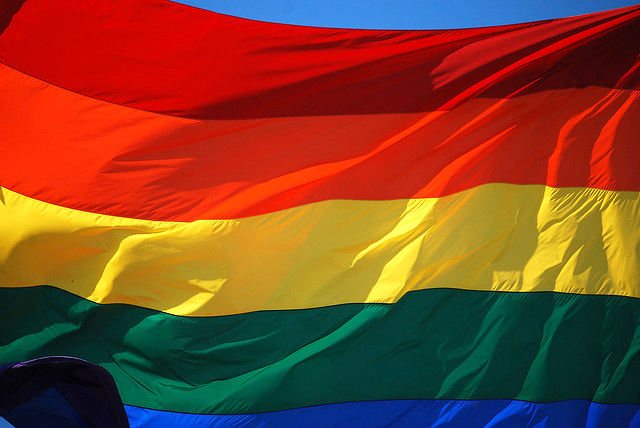
\includegraphics[scale=0.3]{flag_original.png}}
	
	\noindent Marked file:
	
	\centerline{
		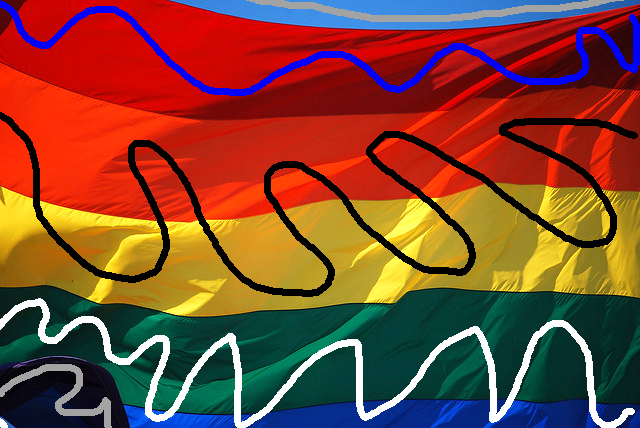
\includegraphics[scale=0.3]{flag_original_marked.png}}
	
	\noindent Weighting function: Y / N
	
	
	\noindent Result: 
	
	\centerline{
		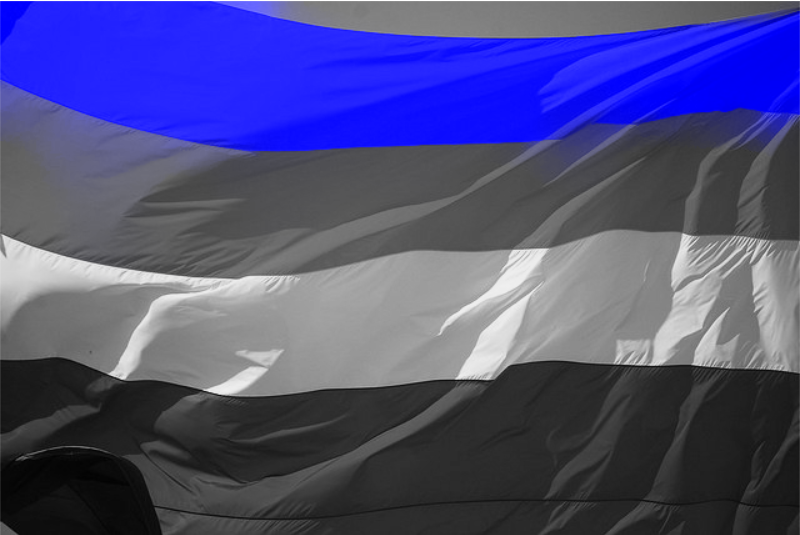
\includegraphics[scale=0.4]{flag_colorized1.png}
		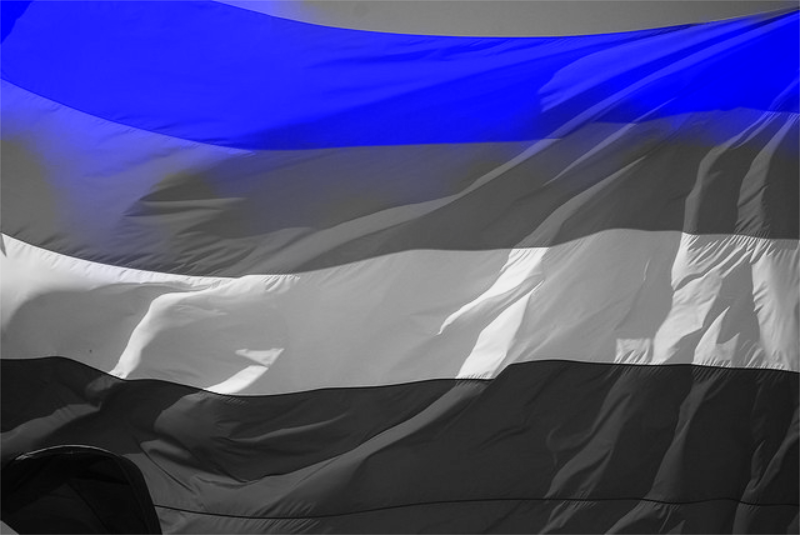
\includegraphics[scale=0.4]{flag_colorized2.png}
	
	}
	
	
	
	\noindent 用时:13.15s / 14.11s
	
	\subsection{存在的缺陷}
	
	\subsubsection{1、颜色不够饱满}
	
	在相同的色度值下,改变Y值,使之从0到1,我们发现生成的颜色并不能满足从纯黑到纯白的变化过程,这是由于YUV转为RGB的保留机制造成的,Y在接近0或接近1时换算成RGB后存在一段溢出值域的范围,即无法表示成颜色,而保留机制的存在会产生一系列较为接近的颜色替代,但无法到达纯黑或纯白。如下图所示,给一张色卡用标准红色上色,结果缺乏纯黑和纯白两端的颜色:
	
	\centerline{
	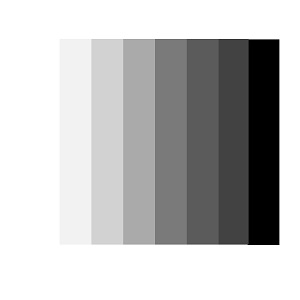
\includegraphics[scale=0.53]{colourcard.png}
	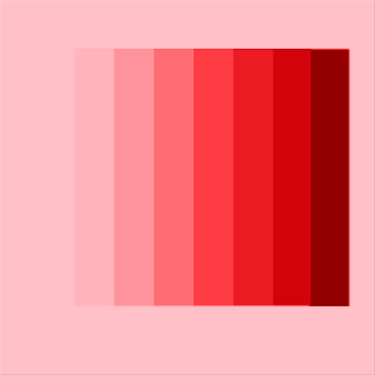
\includegraphics[scale=0.7]{colourcard_colorized.png}}

	因此,在亮度较低的区域(如头发),仅靠棕色一种颜色上色是不够的(左图为上色后的图片,右图为原图):
	
	\centerline{
		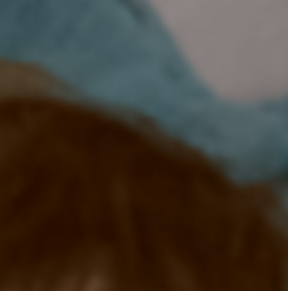
\includegraphics[scale=0.78]{hair1.png}
		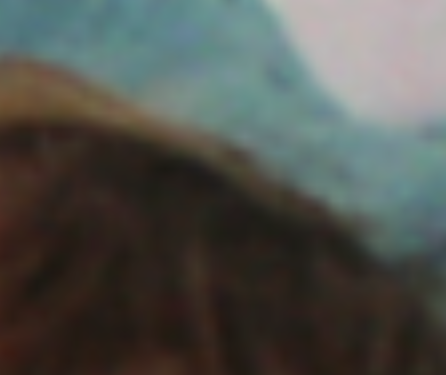
\includegraphics[scale=0.6]{hair2.png}}
	
	解决方法相对比较简单,就是进行强化局部上色,在亮度较低的区域或较高的区域着上黑色或白色,与其它颜色一起拟合剩下的区域,缺点就是可能很难人为判断应该强化上色的区域。
	
	\subsubsection{2、边缘的上色}
	
	边缘是亮度突变的地方,本文的着色方法会在权衡比重后选择一种在边缘两侧两种颜色之间的YUV区间的一种颜色,但在现实生活中,填充边缘的颜色是由多种因素造成的(左图为上色后的图片,右图为原图):
	
	\centerline{
		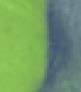
\includegraphics[scale=3]{1.jpg}
		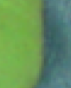
\includegraphics[scale=3.1]{2.png}}
	
	\subsubsection{3、相关性比重函数}
	
	根据0.4.2产生的结果,不难看出相关性函数的溢色较为严重,没有正态分布函数得出的上色图像效果来的好。笔者也进行了多次尝试,仍然不能给出更好的结果。因此笔者也询问了原作者,但暂时还没有得到答复。
	
	\section{参考内容}
	
	\subsubsection{文献:}
	
	\hangafter = 1
	\hangindent 0.5in
	\noindent 
	Levin, A., Lischinski, D., \& Weiss, Y. (2004). Colorization using optimization. In ACM SIGGRAPH 2004 Papers (pp. 689-694).
	
	\noindent Zomet, A., \& Peleg, S. (2002, December). Multi-sensor super-resolution. In Sixth IEEE Workshop on Applications of Computer Vision, 2002.(WACV 2002). Proceedings. (pp. 27-31). IEEE.
	
	\subsubsection{网址:}
	
	\noindent https://github.com/geap/Colorization
	
	\noindent https://blog.csdn.net/u011426016/article/details/103427914
	
\end{document}